
%% bare_jrnl.tex
%% V1.3
%% 2007/01/11
%% by Michael Shell
%% see http://www.michaelshell.org/
%% for current contact information.
%%
%% This is a skeleton file demonstrating the use of IEEEtran.cls
%% (requires IEEEtran.cls version 1.7 or later) with an IEEE journal paper.
%%
%% Support sites:
%% http://www.michaelshell.org/tex/ieeetran/
%% http://www.ctan.org/tex-archive/macros/latex/contrib/IEEEtran/
%% and
%% http://www.ieee.org/

% *** Authors should verify (and, if needed, correct) their LaTeX system  ***
% *** with the testflow diagnostic prior to trusting their LaTeX platform ***
% *** with production work. IEEE's font choices can trigger bugs that do  ***
% *** not appear when using other class files.                            ***
% The testflow support page is at:
% http://www.michaelshell.org/te x/testflow/


%%*************************************************************************
%% Legal Notice:
%% This code is offered as-is without any warranty either expressed or
%% implied; without even the implied warranty of MERCHANTABILITY or
%% FITNESS FOR A PARTICULAR PURPOSE! 
%% User assumes all risk.
%% In no event shall IEEE or any contributor to this code be liable for
%% any damages or losses, including, but not limited to, incidental,
%% consequential, or any other damages, resulting from the use or misuse
%% of any information contained here.
%%
%% All comments are the opinions of their respective authors and are not
%% necessarily endorsed by the IEEE.
%%
%% This work is distributed under the LaTeX Project Public License (LPPL)
%% ( http://www.latex-project.org/ ) version 1.3, and may be freely used,
%% distributed and modified. A copy of the LPPL, version 1.3, is included
%% in the base LaTeX documentation of all distributions of LaTeX released
%% 2003/12/01 or later.
%% Retain all contribution notices and credits.
%% ** Modified files should be clearly indicated as such, including  **
%% ** renaming them and changing author support contact information. **
%%
%% File list of work: IEEEtran.cls, IEEEtran_HOWTO.pdf, bare_adv.tex,
%%                    bare_conf.tex, bare_jrnl.tex, bare_jrnl_compsoc.tex
%%*************************************************************************

% Note that the a4paper option is mainly intended so that authors in
% countries using A4 can easily print to A4 and see how their papers will
% look in print - the typesetting of the document will not typically be
% affected with changes in paper size (but the bottom and side margins will).
% Use the testflow package mentioned above to verify correct handling of
% both paper sizes by the user's LaTeX system.
%
% Also note that the "draftcls" or "draftclsnofoot", not "draft", option
% should be used if it is desired that the figures are to be displayed in
% draft mode.
%
\documentclass[journal]{IEEEtran}
%
% If IEEEtran.cls has not been installed into the LaTeX system files,
% manually specify the path to it like:
% \documentclass[journal]{../sty/IEEEtran}





% Some very useful LaTeX packages include:
% (uncomment the ones you want to load)


% *** MISC UTILITY PACKAGES ***
%
%\usepackage{ifpdf}
% Heiko Oberdiek's ifpdf.sty is very useful if you need conditional
% compilation based on whether the output is pdf or dvi.
% usage:
% \ifpdf
%   % pdf code
% \else
%   % dvi code
% \fi
% The latest version of ifpdf.sty can be obtained from:
% http://www.ctan.org/tex-archive/macros/latex/contrib/oberdiek/
% Also, note that IEEEtran.cls V1.7 and later provides a builtin
% \ifCLASSINFOpdf conditional that works the same way.
% When switching from latex to pdflatex and vice-versa, the compiler may
% have to be run twice to clear warning/error messages.






% *** CITATION PACKAGES ***
%
%\usepackage{cite}
% cite.sty was written by Donald Arseneau
% V1.6 and later of IEEEtran pre-defines the format of the cite.sty package
% \cite{} output to follow that of IEEE. Loading the cite package will
% result in citation numbers being automatically sorted and properly
% "compressed/ranged". e.g., [1], [9], [2], [7], [5], [6] without using
% cite.sty will become [1], [2], [5]--[7], [9] using cite.sty. cite.sty's
% \cite will automatically add leading space, if needed. Use cite.sty's
% noadjust option (cite.sty V3.8 and later) if you want to turn this off.
% cite.sty is already installed on most LaTeX systems. Be sure and use
% version 4.0 (2003-05-27) and later if using hyperref.sty. cite.sty does
% not currently provide for hyperlinked citations.
% The latest version can be obtained at:
% http://www.ctan.org/tex-archive/macros/latex/contrib/cite/
% The documentation is contained in the cite.sty file itself.



% *** GRAPHICS RELATED PACKAGES ***
%
\ifCLASSINFOpdf
  \usepackage[pdftex]{graphicx}
  \usepackage{epstopdf}
   \usepackage{amsmath,amssymb,exscale}

  % declare the path(s) where your graphic files are
   \graphicspath{{./images/}}
  % and their extensions so you won't have to specify these with
  % every instance of \includegraphics
   \DeclareGraphicsExtensions{.pdf,.jpeg,.png}
\else
  % or other class option (dvipsone, dvipdf, if not using dvips). graphicx
  % will default to the driver specified in the system graphics.cfg if no
  % driver is specified.
  % \usepackage[dvips]{graphicx}
  % declare the path(s) where your graphic files are
  % \graphicspath{{../eps/}}
  % and their extensions so you won't have to specify these with
  % every instance of \includegraphics
  % \DeclareGraphicsExtensions{.eps}
\fi
% graphicx was written by David Carlisle and Sebastian Rahtz. It is
% required if you want graphics, photos, etc. graphicx.sty is already
% installed on most LaTeX systems. The latest version and documentation can
% be obtained at: 
% http://www.ctan.org/tex-archive/macros/latex/required/graphics/
% Another good source of documentation is "Using Imported Graphics in
% LaTeX2e" by Keith Reckdahl which can be found as epslatex.ps or
% epslatex.pdf at: http://www.ctan.org/tex-archive/info/
%
% latex, and pdflatex in dvi mode, support graphics in encapsulated
% postscript (.eps) format. pdflatex in pdf mode supports graphics
% in .pdf, .jpeg, .png and .mps (metapost) formats. Users should ensure
% that all non-photo figures use a vector format (.eps, .pdf, .mps) and
% not a bitmapped formats (.jpeg, .png). IEEE frowns on bitmapped formats
% which can result in "jaggedy"/blurry rendering of lines and letters as
% well as large increases in file sizes.
%
% You can find documentation about the pdfTeX application at:
% http://www.tug.org/applications/pdftex





% *** MATH PACKAGES ***
%
%\usepackage[cmex10]{amsmath}
\usepackage{amsfonts}
% A popular package from the American Mathematical Society that provides
% many useful and powerful commands for dealing with mathematics. If using
% it, be sure to load this package with the cmex10 option to ensure that
% only type 1 fonts will utilized at all point sizes. Without this option,
% it is possible that some math symbols, particularly those within
% footnotes, will be rendered in bitmap form which will result in a
% document that can not be IEEE Xplore compliant!
%
% Also, note that the amsmath package sets \interdisplaylinepenalty to 10000
% thus preventing page breaks from occurring within multiline equations. Use:
%\interdisplaylinepenalty=2500
% after loading amsmath to restore such page breaks as IEEEtran.cls normally
% does. amsmath.sty is already installed on most LaTeX systems. The latest
% version and documentation can be obtained at:
% http://www.ctan.org/tex-archive/macros/latex/required/amslatex/math/





% *** SPECIALIZED LIST PACKAGES ***
%
\usepackage{algorithm}
\usepackage{algorithmic}
\usepackage{lipsum}
\usepackage{multirow}

% algorithmic.sty was written by Peter Williams and Rogerio Brito.
% This package provides an algorithmic environment fo describing algorithms.
% You can use the algorithmic environment in-text or within a figure
% environment to provide for a floating algorithm. Do NOT use the algorithm
% floating environment provided by algorithm.sty (by the same authors) or
% algorithm2e.sty (by Christophe Fiorio) as IEEE does not use dedicated
% algorithm float types and packages that provide these will not provide
% correct IEEE style captions. The latest version and documentation of
% algorithmic.sty can be obtained at:
% http://www.ctan.org/tex-archive/macros/latex/contrib/algorithms/
% There is also a support site at:
% http://algorithms.berlios.de/index.html
% Also of interest may be the (relatively newer and more customizable)
% algorithmicx.sty package by Szasz Janos:
% http://www.ctan.org/tex-archive/macros/latex/contrib/algorithmicx/




% *** ALIGNMENT PACKAGES ***
%
%\usepackage{array}
% Frank Mittelbach's and David Carlisle's array.sty patches and improves
% the standard LaTeX2e array and tabular environments to provide better
% appearance and additional user controls. As the default LaTeX2e table
% generation code is lacking to the point of almost being broken with
% respect to the quality of the end results, all users are strongly
% advised to use an enhanced (at the very least that provided by array.sty)
% set of table tools. array.sty is already installed on most systems. The
% latest version and documentation can be obtained at:
% http://www.ctan.org/tex-archive/macros/latex/required/tools/


%\usepackage{mdwmath}
%\usepackage{mdwtab}
% Also highly recommended is Mark Wooding's extremely powerful MDW tools,
% especially mdwmath.sty and mdwtab.sty which are used to format equations
% and tables, respectively. The MDWtools set is already installed on most
% LaTeX systems. The lastest version and documentation is available at:
% http://www.ctan.org/tex-archive/macros/latex/contrib/mdwtools/


% IEEEtran contains the IEEEeqnarray family of commands that can be used to
% generate multiline equations as well as matrices, tables, etc., of high
% quality.


%\usepackage{eqparbox}
% Also of notable interest is Scott Pakin's eqparbox package for creating
% (automatically sized) equal width boxes - aka "natural width parboxes".
% Available at:
% http://www.ctan.org/tex-archive/macros/latex/contrib/eqparbox/





% *** SUBFIGURE PACKAGES ***
%\usepackage[tight,footnotesize]{subfigure}
% subfigure.sty was written by Steven Douglas Cochran. This package makes it
% easy to put subfigures in your figures. e.g., "Figure 1a and 1b". For IEEE
% work, it is a good idea to load it with the tight package option to reduce
% the amount of white space around the subfigures. subfigure.sty is already
% installed on most LaTeX systems. The latest version and documentation can
% be obtained at:
% http://www.ctan.org/tex-archive/obsolete/macros/latex/contrib/subfigure/
% subfigure.sty has been superceeded by subfig.sty.



%\usepackage[caption=false]{caption}
%\usepackage[font=footnotesize]{subfig}
% subfig.sty, also written by Steven Douglas Cochran, is the modern
% replacement for subfigure.sty. However, subfig.sty requires and
% automatically loads Axel Sommerfeldt's caption.sty which will override
% IEEEtran.cls handling of captions and this will result in nonIEEE style
% figure/table captions. To prevent this problem, be sure and preload
% caption.sty with its "caption=false" package option. This is will preserve
% IEEEtran.cls handing of captions. Version 1.3 (2005/06/28) and later 
% (recommended due to many improvements over 1.2) of subfig.sty supports
% the caption=false option directly:
%\usepackage[caption=false,font=footnotesize]{subfig}
%
% The latest version and documentation can be obtained at:
% http://www.ctan.org/tex-archive/macros/latex/contrib/subfig/
% The latest version and documentation of caption.sty can be obtained at:
% http://www.ctan.org/tex-archive/macros/latex/contrib/caption/




% *** FLOAT PACKAGES ***
%
%\usepackage{fixltx2e}
% fixltx2e, the successor to the earlier fix2col.sty, was written by
% Frank Mittelbach and David Carlisle. This package corrects a few problems
% in the LaTeX2e kernel, the most notable of which is that in current
% LaTeX2e releases, the ordering of single and double column floats is not
% guaranteed to be preserved. Thus, an unpatched LaTeX2e can allow a
% single column figure to be placed prior to an earlier double column
% figure. The latest version and documentation can be found at:
% http://www.ctan.org/tex-archive/macros/latex/base/

\usepackage[textsize=footnotesize]{todonotes}
\usepackage{times}

%\usepackage{stfloats}
% stfloats.sty was written by Sigitas Tolusis. This package gives LaTeX2e
% the ability to do double column floats at the bottom of the page as well
% as the top. (e.g., "\begin{figure*}[!b]" is not normally possible in
% LaTeX2e). It also provides a command:
%\fnbelowfloat
% to enable the placement of footnotes below bottom floats (the standard
% LaTeX2e kernel puts them above bottom floats). This is an invasive package
% which rewrites many portions of the LaTeX2e float routines. It may not work
% with other packages that modify the LaTeX2e float routines. The latest
% version and documentation can be obtained at:
% http://www.ctan.org/tex-archive/macros/latex/contrib/sttools/
% Documentation is contained in the stfloats.sty comments as well as in the
% presfull.pdf file. Do not use the stfloats baselinefloat ability as IEEE
% does not allow \baselineskip to stretch. Authors submitting work to the
% IEEE should note that IEEE rarely uses double column equations and
% that authors should try to avoid such use. Do not be tempted to use the
% cuted.sty or midfloat.sty packages (also by Sigitas Tolusis) as IEEE does
% not format its papers in such ways.


%\ifCLASSOPTIONcaptionsoff
%  \usepackage[nomarkers]{endfloat}
% \let\MYoriglatexcaption\caption
% \renewcommand{\caption}[2][\relax]{\MYoriglatexcaption[#2]{#2}}
%\fi
% endfloat.sty was written by James Darrell McCauley and Jeff Goldberg.
% This package may be useful when used in conjunction with IEEEtran.cls'
% captionsoff option. Some IEEE journals/societies require that submissions
% have lists of figures/tables at the end of the paper and that
% figures/tables without any captions are placed on a page by themselves at
% the end of the document. If needed, the draftcls IEEEtran class option or
% \CLASSINPUTbaselinestretch interface can be used to increase the line
% spacing as well. Be sure and use the nomarkers option of endfloat to
% prevent endfloat from "marking" where the figures would have been placed
% in the text. The two hack lines of code above are a slight modification of
% that suggested by in the endfloat docs (section 8.3.1) to ensure that
% the full captions always appear in the list of figures/tables - even if
% the user used the short optional argument of \caption[]{}.
% IEEE papers do not typically make use of \caption[]'s optional argument,
% so this should not be an issue. A similar trick can be used to disable
% captions of packages such as subfig.sty that lack options to turn off
% the subcaptions:
% For subfig.sty:
% \let\MYorigsubfloat\subfloat
% \renewcommand{\subfloat}[2][\relax]{\MYorigsubfloat[]{#2}}
% For subfigure.sty:
% \let\MYorigsubfigure\subfigure
% \renewcommand{\subfigure}[2][\relax]{\MYorigsubfigure[]{#2}}
% However, the above trick will not work if both optional arguments of
% the \subfloat/subfig command are used. Furthermore, there needs to be a
% description of each subfigure *somewhere* and endfloat does not add
% subfigure captions to its list of figures. Thus, the best approach is to
% avoid the use of subfigure captions (many IEEE journals avoid them anyway)
% and instead reference/explain all the subfigures within the main caption.
% The latest version of endfloat.sty and its documentation can obtained at:
% http://www.ctan.org/tex-archive/macros/latex/contrib/endfloat/
%
% The IEEEtran \ifCLASSOPTIONcaptionsoff conditional can also be used
% later in the document, say, to conditionally put the References on a 
% page by themselves.





% *** PDF, URL AND HYPERLINK PACKAGES ***
%
%\usepackage{url}
% url.sty was written by Donald Arseneau. It provides better support for
% handling and breaking URLs. url.sty is already installed on most LaTeX
% systems. The latest version can be obtained at:
% http://www.ctan.org/tex-archive/macros/latex/contrib/misc/
% Read the url.sty source comments for usage information. Basically,
% \url{my_url_here}.





% *** Do not adjust lengths that control margins, column widths, etc. ***
% *** Do not use packages that alter fonts (such as pslatex).         ***
% There should be no need to do such things with IEEEtran.cls V1.6 and later.
% (Unless specifically asked to do so by the journal or conference you plan
% to submit to, of course. )


% correct bad hyphenation here
\hyphenation{op-tical net-works semi-conduc-tor}

\usepackage{setspace}
\newcommand{\stodo}[2][]
{\todo[caption={#2}, #1]
{\begin{spacing}{1.0}#2\end{spacing}}}


\begin{document}
%
% paper title
% can use linebreaks \\ within to get better formatting as desired
\title{A Dynamic Load-Balancing Algorithm for Heterogeneous GPU Clusters}
%
%
% author names and IEEE memberships
% note positions of commas and nonbreaking spaces ( ~ ) LaTeX will not break
% a structure at a ~ so this keeps an author's name from being broken across
% two lines.
% use \thanks{} to gain access to the first footnote area
% a separate \thanks must be used for each paragraph as LaTeX2e's \thanks
% was not built to handle multiple paragraphs
%

\author{Luis~Sant'Ana,~\IEEEmembership{CMCC-UFABC}
        Daniel~Cordeiro,~\IEEEmembership{DCC-USP}
        and~Raphael~Camargo,~\IEEEmembership{CMCC-UFABC}% <-this % stops a space

\thanks{Luis Sant'Ana is with the Center Mathematics, Computation and Cognition, Federal Uniersity of ABC, Santo Andr\'{e}, SP, Brazil e-mail: luis.ana@ufabc.edu.br}% <-this % stops a space
\thanks{Daniel Cordeiro is with the Department of Computer Science, University of S\~{a}o Paulo, S\~{a}o Paulo, SP, Brazil e-mail: danielc@ime.usp.br }% <-this % stops a space
\thanks{Raphael Carmargo is with the Center Mathematics, Computation and Cognition, Federal Uniersity of ABC, Santo Andr\'{e}, SP, Brazil e-mail: raphael.camargo@ufabc.edu.br}}

% note the % following the last \IEEEmembership and also \thanks - 
% these prevent an unwanted space from occurring between the last author name
% and the end of the author line. i.e., if you had this:
% 
% \author{....lastname \thanks{...} \thanks{...} }
%                     ^------------^------------^----Do not want these spaces!
%
% a space would be appended to the last name and could cause every name on that
% line to be shifted left slightly. This is one of those "LaTeX things". For
% instance, "\textbf{A} \textbf{B}" will typeset as "A B" not "AB". To get
% "AB" then you have to do: "\textbf{A}\textbf{B}"
% \thanks is no different in this regard, so shield the last } of each \thanks
% that ends a line with a % and do not let a space in before the next \thanks.
% Spaces after \IEEEmembership other than the last one are OK (and needed) as
% you are supposed to have spaces between the names. For what it is worth,
% this is a minor point as most people would not even notice if the said evil
% space somehow managed to creep in.



% The paper headers
\markboth{IEEE/ACM CCGrid 2015 
15th IEEE/ACM International Symposium on Cluster, Cloud and Grid Computing}%
{Shell \MakeLowercase{\textit{et al.}}:  Dynamic Load-Balancing}
% The only time the second header will appear is for the odd numbered pages
% after the title page when using the twoside option.
% 
% *** Note that you probably will NOT want to include the author's ***
% *** name in the headers of peer review papers.                   ***
% You can use \ifCLASSOPTIONpeerreview for conditional compilation here if
% you desire.




% If you want to put a publisher's ID mark on the page you can do it like
% this:
%\IEEEpubid{0000--0000/00\$00.00~\copyright~2007 IEEE}
% Remember, if you use this you must call \IEEEpubidadjcol in the second
% column for its text to clear the IEEEpubid mark.



% use for special paper notices
%\IEEEspecialpapernotice{(Invited Paper)}




% make the title area
\maketitle


\begin{abstract}
%\boldmath
The use of GPU clusters for scientific applications is becoming more widespread,
with applications in areas such as physics, chemistry and bioinformatics. These
clusters can be highly heterogenous, composed of several models of CPUs and
GPUs, that could be used together to execute these applications. To use these
heterogeneous devices in an efficient manner, it is necessary to load-balance
the application task sizes among the GPUs and CPUs, minimizing the execution
time of the application.

We propose an algorithm for dynamic load balancing in heterogeneous GPU clusters
that determines the execution profile of tasks on each device in runtime. This
profile is used to find the best distribution of task sizes among devices. We
implemented the algorithm in the StarPU framework and compared its performance
with existing load-balancing algorithms, using applications from linear algebra,
stock markets and bioinformatics.

\end{abstract}
% IEEEtran.cls defaults to using nonbold math in the Abstract.
% This preserves the distinction between vectors and scalars. However,
% if the journal you are submitting to favors bold math in the abstract,
% then you can use LaTeX's standard command \boldmath at the very start
% of the abstract to achieve this. Many IEEE journals frown on math
% in the abstract anyway.

% Note that keywords are not normally used for peerreview papers.
\begin{IEEEkeywords}
parallel computing, distribuited systems, GPU cluster, GPGPU.
\end{IEEEkeywords}


% For peer review papers, you can put extra information on the cover
% page as needed:
% \ifCLASSOPTIONpeerreview
% \begin{center} \bfseries EDICS Category: 3-BBND \end{center}
% \fi
%
% For peerreview papers, this IEEEtran command inserts a page break and
% creates the second title. It will be ignored for other modes.
\IEEEpeerreviewmaketitle

\section{Introduction}

% You must have at least 2 lines in the paragraph with the drop letter
% (should never be an issue)
%\IEEEPARstart{T}{he} 

% RYC1029: Luis -> colocar referências mais recentes.
The use of GPUs (Graphics Processing Units) is becoming increasingly popular
among developers and users of applications that have high computational demands
and can benefit from a large degree of parallelism~\cite{gpu2}. Among these
applications we can include fluid mechanics~\cite{fluid2}, visualization
science~\cite{visualization2}, machine learning~\cite{learning2},
bioinformatics~\cite{bioinformatica2} and neural networks~\cite{neural}.

% RYC1029: Luis -> incluir referências de bibliotecas, como da nVidia e outras
Modern GPUs can have thousands of simple floating point units (FPUs) that,
combined, can have a computational power several times superior to traditional
CPUs. The main drawback is the difficult in optimizing GPU code, specially
considering the architectural differences among different GPUs, with changes in
the distribution of cores, shared memory, presence of cache, among others. But
libraries for several classes of applications and algorithms are now available,
facilitating the deevlopment process~\cite{}.

Computationally demanding applications may also benefit from the usage of
multiple GPUs, normally distributed on several machines, which are called GPU
clusters~\cite{raphael, cluster}. The development of applications for these
clusters is more complex, since it requires the management of the multiple
memory spaces, one for each GPU in the cluster, in addition to the main memory
of the each node. This management includes transferring data between these
memory spaces and ensuring the consistency of data. 

There are several efforts by the scientific community for the creation of new
programming models~\cite{appCientificas, wave} and frameworks~\cite{snucl, Flat,
  starpu}, for facilitating the developement of GPU cluster
applications. However, the combination of CUDA (Compute Unified Device
Architecture) and MPI (Message Passing Interface) is still the standard choice
to develop applications for GPU clusters.

High-performance GPU clusters are typically \emph{homogeneous}, containing nodes
and GPUs with the same configuration. Homogeneity facilitates the development of
applications, since they can be optimized just for a single
architecture. Moreover, if the application has exclusive access to the nodes,
load-balancing is simpler, since the same task size, or number of tasks, can be
allocateds to each node. But homogeneity can be difficult to maintain in a
context where a new generation of hardware is launched every couple of years. In
this case, joining heterogeneous machines can increase the available
computational power to cluster users.

Another scenario where heterogeneity is more common is when connecting machines
from several researchers groups using a standard Ethernet network. This enables
a large amount of computing power from commodity hardware that could be
efficiently used by application with low communication demands. These machines
could be used by these applications outside the work time and the aquisition
cost and space demand for this commodity-hardware GPU cluster would be almost
zero.

Developing a load-balancing mechanism that works efficiently for all kinds of
applications is difficult. With two or more GPUs (or CPUs), this problem is
strictly equivalent to the classic problem of minimizing the maximum completion
time of all tasks (makespan), which is known to be NP-hard \cite{GaJo1979}. An
efficient load-balancing scheme must be considered on case by case basis. For
example, there are several types of data-parallel
applications~\cite{Gropp:1992uq} that could be divided using domain
decomposition. Several scientific applications fit into this group, including
applications in bioinformatics~\cite{bioinformatica2}, neural
networks~\cite{neural}, chemistry, physics and materials science.

When using homogeneous clusters, data can be distributed among the available
GPUs using tasks of the same size. However, with heterogeneous GPUs, this
distribution is more difficult. There are several existing GPU architectures,
such as \emph{Tesla},​ \emph{Fermi}, \emph{Kepler} and \emph{Maxwell}. These
architectures have different organizations of FPUs (Floating-point Unit),
caches, shared memory and memory speeds. Even for GPUs with the same
architectures, their characteristics can vary considerably.

A division of the load based on simple heuristics, such as a the number of cores
in the GPU, is not effective and can be worse than a simple homogeneous
division~\cite{raphael}. Also, different architectures require different
low-level optimizations and a code could have been better optimized for one
architecture. Finally, GPUs clusters normally have high-end CPUs in addition to
the GPUs, and these CPUs can used by the applications.

% RYC2910: Comentei o texto abaixo, pois no momento não dmos suporte a múltiplos
%tipos de tarefas. Acho que o próximo passo natural seria termos suporte a
%colocar labels nas tarefas e criarmos perfis para cada tipo de tarefa.
%
%; for instance, to execute parts of the code which cannot be
%coded efficiently using the Single Instruction Multiple Thread (SIMT) model of
%GPUs.

The main task of the load-balancing mechanism is to devise the best data
division amont the GPUs. A possible approach is to determine the performance
profiles for each GPU type and application task and use it to determine the
amount of work given to each GPU. This profiling can be done statically, before
application execution~\cite{raphael}, or dynamically, during application
execution~\cite{acosta, HDSS}. Another solution is to use simple algorithms for
task dispatching, such as the greedy algorithm from StarPU~\cite{starpu}, where
tasks are dispatched to the devices as soon as they become available.

In this work we propose a novel adaptive algorithm for dynamic load balancing of
data-parallel applications in heterogeneous GPU clusters. The algorithm uses
runtime task execution time measurements to create a performance model for each
device (CPU or GPU). The algorithm dynamically adjust the size of data blocks
allocated to each device based on this model. We compared the proposed algorithm
with static~\cite{raphael} and dynamic (HDSS)~\cite{HDSS} algorithms and with
the standard StarPU greedy algorithm.

% The very first letter is a 2 line initial drop letter followed
% by the rest of the first word in caps.
% 
% form to use if the first word consists of a single letter:
% \IEEEPARstart{A}{demo} file is ....
% 
% form to use if you need the single drop letter followed by
% normal text (unknown if ever used by IEEE):
% \IEEEPARstart{A}{}demo file is ....
% 
% Some journals put the first two words in caps:
% \IEEEPARstart{T}{his demo} file is ....
% 
% Here we have the typical use of a "T" for an initial drop letter
% and "HIS" in caps to complete the first word.

%%%%%%%%%%%%%%%%%%%%%%%%%%%%%%%%%%%%%%%%%%%%%%%%%%%%%%%%%%%%%%%%%%%%%%%%%%%%

\section{Related Work}

A proposed solution for load balancing in distributed systems is to divide the
tasks among CPUs according to a weight factor representing the processing speed
of each processor. Early approaches used fixed weight factors determined at
compile time with limited success~\cite{Hummel}. But these weight factors are
difficult to determine in heterogeneous GPUs, due to the architectural
differences that affect the performance.

The problem of load balancing in heterogeneous GPUs, began to be studied
recently. One proposal was the usage of a static algorithm that determines the
distribution before the execution of the application, using profiles from
previous executions~\cite{raphael}. The algorithm uses these profiles to find
the distribution of data that minimizes the execution time of the application,
ensuring that all GPUs to spend same amount of time performing the processing of
kernels. The algorithm was evaluated using a large-scale neural network
simulation. Its main drawback is that since it is static, an initial unbalanced
distribution cannot be djusted in runtime. Another problem is that it require
preivous executions of the appliction in the target deveices to determine its
exexuction profiles. Finally, it does not consider the case where application
behavior changes with the parameters. A dynamic algorithm, like the one that we
propose, do not have these limitations.

% RYC1029: Luis -> Não está muito claro como é feita a coordenação aqui. Cada
% processador realiza sua própria distribuição, mas de algum modo os processos
% precisam chegar num acordo de qual pedaço vai para qual processador. Precisa
% verificar melhor como funciona o algoritmo. Outro ponto é sobre como a
% distribuição é feita. Dizer apenas que o tempo de execução é comparado não é
% suficiente. É preciso dizer como esta diferença é utilizada. Como a descrição
% do algoritmo não é clara, a comparação com nosso algoritmo está ruim. Por que
% é melhor ser centralizado e usar as curvas para fazer o load-balancing? Quais
% são as desvantagens do algoritmo de Acosta? Veja minha comparação com o HDSS.
Acosta \emph{et al.}~\cite{acosta} proposed a dynamic load balancing algorithm
that interactively finds a good distribution of work between GPUs during
application execution. It uses a decentralized scheme in which synchronizations
are done at each iteration to determine whether there is a need to rebalance the
load. Each process, representing a single GPU, performs a redistribution of
workload according to the size of the assigned task and the capabilities of the
GPU. Load balancing is obtained by comparing the execution time of the current
task for each GPU with the redistribution of the subsequent task. If this time
difference reaches a threshold, a load redistribution is triggered. Our
algorithm is different because is centralized and it creates curves for each
processing unit, and based on these curves performs the load balancing.

The Heterogeneous Dynamic Self-Scheduler (HDSS)~\cite{HDSS} is a dynamic
load-balancing algorithm for heterogenous GPU clusters. It is divided in two
phases. The first is the adaptive phase, where it determines weights that
reflect the speed of each GPU, similarly to Hummel \emph{et al.}~\cite{Hummel},
but performed dynamically and using profiling data. A performance curve with the
FLOPs per second for each task size is created for each GPU. The weights is
determined based on logarithmic fits on the curves.  These weights are used
during the second phase, called completion phase, where it divides the remaining
iterations among the GPUs based on their relative weights. It starts allocating
larger block sizes to the GPUs, decreasing their size as the execution
progresses. An important drawback of HDSS is that the weight model based on
logarithmic curves is valid only for GPUs, where the number of FLOPs per second
stabilizes with larger tasks. Also, after the weights are determined they cannot
be changed. We use an execution model that fits for both GPUs, CPUs and other
device types. Moreover, we use the complete performance models, instead of a
single number, resulting in a better load-distribution. Finally, we use the task
execution time data from all the execution, permiting later adjustments in the
performance models of the devices.


%%%%%%%%%%%%%%%%%%%%%%%%%%%%%%%%%%%%%%%%%%%%%%%%%%%%%%%%%%%%%%%%%%%%%%%%%%%%

\section{Proposed Algorithm}

In a typical data-parallel application, the application data is divided among
the threads in a process called domain decomposition~\cite{Gropp:1992uq}. The
threads then simultaneously process their part of the data and this processing
can be on single or multiple steps, dependending on the task sizes. After
finishing, the threads merge the processed results, and the application
terminates or continues to the next phase of computing. The task of our
load-balancing algorithm is determining the size of the data block assigned to
each GPU and CPU in the system. We will use the term processor to mean a single
CPU or GPU.

%RYC1029: Acho que aqui fica melhor se os paragraph forem alterados para
%subsection.
\vspace{0.2cm}
\paragraph*{Overview} The algorithm has three parts, which are: (1) processor 
performance modeling, where a performance model for each processor is determined
during application execution based on task execution times; (2) optimal block
size selection, where, based on the performance model, the algorithm determines
the best distribution of block size among the processors; and (3) re-balancing,
where the algorithm recalculates the optimal block sizes when the difference in
execution time by different processors is larger than a threshold.

% RYC1029: Aqui um figura estilo fluxograma seria interessante
%
%         |
%         v
% Performance Modeling <------
%         |                  |
%         v                  |
% Block Size Selection   Rebalancing 
%         |                  |
%         v                  |
%  -> Task Execution         |
%  |      |                  |  
%  -- Thresholds checking ----

\begin{figure}[!t]
	\centering
			\includegraphics[scale=0.36]{CPUVersusGPULinear2.pdf} 				
	\caption{GPU and CPU processing times for different block sizes.}
	\label{fig: CPUVersusGPU1}
\end{figure}


\vspace{0.2cm}
% RYC1029: Modifiquei toda a seção. Veja se o que escrevi está correto,
% especialmente a parte do coeficiente de correlação.
\paragraph*{Processor performance modelling.} In this part, the algorithm 
constructs a function $P_p[x]$, which represents the execution time of a block
of data of size $x$ on processor $p$. For this, it executes blocks of different
sizes on each processor and interpolate the curve that better fits these points.

A block of size $initialBlockSize$, defined by the user, is initially allocated
and executed on each processor. After executing the first block, the algorithm
selects the processor with the earliest finish time $t_f$ and double the block
size for this processor. For other processors, with finish times $t_k$, we
select blocks of size $initialBlockSize * t_k / t_f$. This procedure is repeated
until generating four points per curve. This process corresponds to (1) in
Figure~\ref{fig: algoritmo}, which shows a schematic view of processor
performance modelling part.

The algorithm then follows the step (2) of Figure~\ref{fig: algoritmo}, where it
tries to fit a curve in the existing points using the least squares fitting
method. If the coefficient of determination is greater than 0.7 for all
processors, the algorithm considers the fit as good enough and finishes this
phase. Otherwise, it generates more points in the curve following the previous
procedure.
 

% RYC1029: Cade o texto onde você explica os tipos de funções e combinações que
% usadas no fitting??? Não tínhamos discutido este ponto e você incluído na
% qualificação?
We find best fit curves by the method of \textit{least squares}, using a
function of the form $f(x) = a x - b$.

Figure~\ref{fig: CPUVersusGPU1} shows sample processing time measurements for a
GPU and a CPU for different block sizes and two applications. We can see that
the curves can be approximated by different types of functions. 
% RYC1029: Colocar as funções que aproximaram cada gráfico.

\begin{figure}[!t]
	\centering
	\includegraphics[scale=0.33]{diagramaAlgoritmo.pdf} 
	\caption{Summary of the algorithm}
	\label{fig: algoritmo}
\end{figure}

% RYC1029: A Figura 2 está com erros. Seria melhor ela representar apenas a
% parte da modelagem de desempenho, dado que ela está nesta seção. Eu juntaria a
% parte (1) com a (2), que é repetida por 4 vezes e só então que prossegue para
% a (3) e (4), que eu juntaria em um item só (3) + (4). Se na (4) o erro das
% funções for menor que um limiar, esta parte termina. Se não for, volta para o
% passo (2). Além disso, essa figura da parte (1) + (2) não ajuda em muita
% coisa. Precisaria repensar como deixá-la melhor e de um jeito que ajude o
% leitor. Passei a descrição da figura para junto do texto explicando o
% algoritmo.



%Using a search method, a solution is found, with the restriction time. The time
%requires to be the same for all processors. The result is block of optimum
%size. If the cluster undergoes a change in behavior, and the time difference
%among the processors exceeds a threshold, the process and the calculation is
%redone.


\begin{algorithm}

\caption{Processor performance model}
\label{algModel}

\begin{algorithmic}		

\STATE \textbf{function}~determineModel()

\STATE $blockSizeList \leftarrow initialBlockSize;$
\WHILE{$fitValues.error \geq 0.5$}
		\STATE $finishTimes$ = executeTasks($blockSizeList$);
	        \STATE $blockSizeList$ = evaluateNextBlockSizes($finishTimes$);
		\STATE $fitValues$ = determineCurveProcessor();
\ENDWHILE

return $fitValues$;

\end{algorithmic}
\end{algorithm}

% RYC1029: O erro é 0.5 ou 0.7? No texto anterior estava 0.7 e no algoritmo está
% 0.5

The steps of this phase are shown in Algorithm~\ref{algModel}, which is executed
in a single node, called master node. Variable $blockListSize$ contains the size
of the blocks assigned to each processor and is initialized with
$initialBlockSize$, which is defined by the user. Variable $fitValues$ contains
results from the last least square fitting, including the $error$ in the
fitting, which is initialized as $+\infty$. In the main loop, while the error is
larger than a predefined value, the function sends a chunk of data for each
processor and obtains the finish time for each processor. After all processors
finish their executions, it determine the block sizes for the next iteration,
based on their finish times. Finally, it tries to fit model curves to each
processor and receives the fitting results.

\vspace{0.2cm}
\paragraph*{Optimal block size selection} In this part our algorithm determines 
the optimal block size for each processor with the objective of providing blocks
with the same execution time on each processor.

Consider we have $n$ processors and a input data size $Z$. The algorithm assigns
a data chunk of size $x^g$ for each processor $g=1,...,n$, corresponding a
fraction of input data, such that $\sum_{g=1}^n x^g = Z$. We denote as
$E^g(x^g)$ the execution time of task $E$ in the processor $g$, for input of
size $x^g$. To distribute the work among the processors, we find a set of values
	
\begin{equation}
	X = \{ x^g \in \mathbb{R}:[0,1] / \sum_{g=1}^n x^g = Z \}
	\label{eq: totalResultado}
\end{equation}

that minimizes $E_1(x_1)$ while satisfying the constraint

\begin{equation}
	E_{1} = E_{2} = ...= E_{n}
	\label{eq: Restricao}
\end{equation}

which represents that all processors should spend the same amount of time
performing the processing. To determine the set of values $x$, we solve the
system of fitted curves for all processors, determined in the performance
modelling part, and given by:

\begin{equation}
	\left\lbrace
	\begin{array}{ll}
		\displaystyle E_{1} = f(x_{1})  \\
		\displaystyle E_{2} = f(x_{2})   \\
		\displaystyle E_{n} = f(x_{n}) 
		\label{eq: system}
	\end{array}
	\right.
\end{equation}

The equations system is solved applying an interior point line search filter
method~\cite{point}, which finds the minimum solution of a convex equation set,
subject to a set of constraints, by transversing the interior points of its
feasible region.

% RYC1029: Temos no começo uma grande quantidade de dados, pegamos uma parte
% destes dados Z e distribuimos entre os processadores. Como este Z é
% determinado? Pegamos uma porcentagem do total de dados? Usa-se valores que
% estão dentro dos valores medidos na parte de performance modelling?

\vspace{0.2cm}
\paragraph*{Execution and Rebalancing}  

After determining the task sizes, the scheduler sends a block of the selected
size $x_i$ for each processor $i$. When a processor finishes executing a task,
it requests another task of the same size. The processors then continue the
execution asynchronously, until completing all the tasks.

% RYC1029: Luis -> completar o XXX abaixo.
The scheduler also monitors the finish time of each task. If the difference in
finishing times $t_i$ and $t_j$ between any two tasks of processors $i$ and $j$
goes above a threshold, the rebalancing process is executed. Small thresholds
may cause excessive rebalancing while large thresholds may tolerate larger
imbalances that will cause processor idlenesses. The threshold is determined
empirically, but values of about XXX\% of the execution time of a single value
resulted in a good tradeoff.

During the rebalancing, the scheduler synchronizes the processors and apply the
processor performance modelling algorithm to fit the best curves for the
functions $P_p[x]$ updated with the execution times. The optimal block size
selection routine is then applied to determine new block sizes $x_i$ for each
processor $i$.

\begin{figure}[!t]
	\centering
			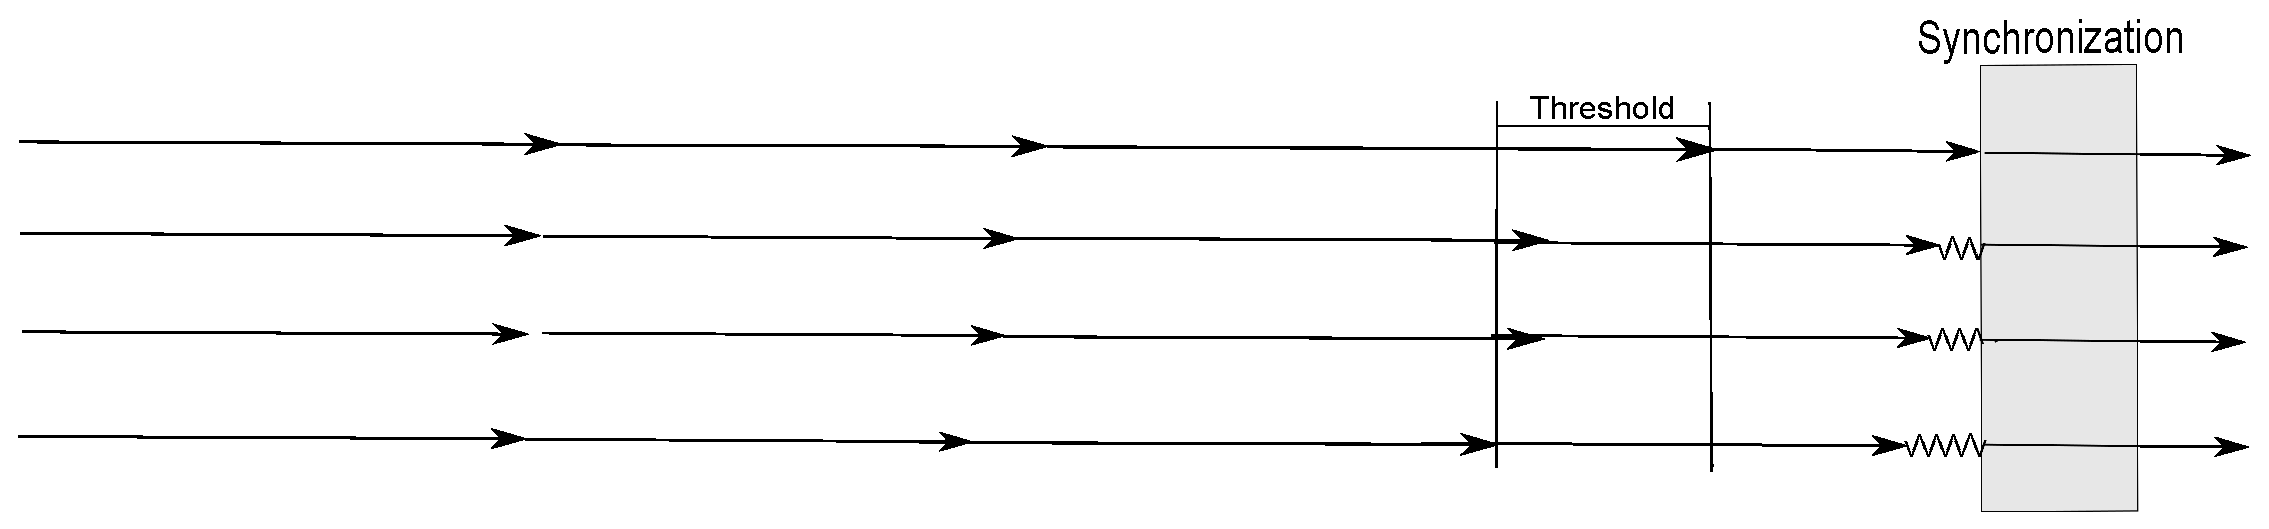
\includegraphics[scale=0.24]{DiagramaArtigo.eps}
	\caption{Execution of tasks by four processors. The finish time
          difference of two tasks was above a threshold, which caused a
          rebalancing of the task sizes.}
	\label{fig:Diagrama}
\end{figure}

% RYC1029: A figura ainda está toda torta, com as tarefas demorando tempos
% aleatórios para executar. Capriche mais na figura, fazendo os tempos de
% execução de cada tarefa proporcional, assim como o aumento do erro. Também
% precisa colocar uma seta no início de cada linha e uma logo depois da
% sincronização. Também precisa incluir onde o algoritmo de rebalancemanto é
% executado.

Figure~\ref{fig:Diagrama} shows a diagram of execution of four processors, where
each arrow indicates the start of a task execution. The tasks start
synchronized, but their finishes times start to diverge until the differences
reaches a threshold. In this case, all threads are synchronized, and the new
task sizes are recalculated for each processors. The task executions then
restart.

\vspace{0.2cm}
\paragraph*{Complete algorithm} 

Algorithm~\ref{alg1} shows the pseudo-code of the scheduling algorithm. The
$determineModel$ function, shown in Algorithm~\ref{algModel} returns the
performance model for each processor into variable $fitValues$. The algorithm
then solves the system of equations contained in $fitValues$ to determine the
best distribution $X$ of task sizes for each processor.

\begin{algorithm}

\caption{Complete dynamic algorithm}
\label{alg1}

\begin{algorithmic}		

\STATE \textbf{function} dynamic()

\STATE $fitValues$ = determineModel()
\STATE $X$ = solveEquationSystem($fitValues$);

\WHILE{there is data}

	\STATE $finishTimes$ = executeTasks($X$);
	\IF {$ $maxDifference($finishTimes$)$ \geq threshold$}
		\STATE $fitValues$ = determineCurveProcessor();
                \STATE $X$ = solveEquationSystem($fitValues$);
                \STATE synchronize();
    	\ENDIF
\ENDWHILE

\end{algorithmic}
\end{algorithm}

% RYC1029: Este algoritmo está errado, pois ele considera que a execução das
% tarefas é síncrona. O algoritmo que você implementou provavelmente é baseado
% em eventos (término de tarefas). Você precisa fazer o mesmo aqui. Em seguida,
% é preciso alterar o texto para refletir estas mudanças.

The main loop repeats while there is still data for processing. It distributes
tasks of different sizes for each processor in the system, obtaining the finish
times for each task execution. It then checks if the maximum difference between
the finish tasks is above a defined threshold. If the threshold is reached, the
algorithm fits new curves for each processor performance model and solve the
system of equations to determine a new distribution of tasks sizes for each
processor.

%%%%%%%%%%%%%%%%%%%%%%%%%%%%%%%%%%%%%%%%%%%%%%%%%%%%%%%%%%%%%%%%%%%%%%%%%%%

\section{Implementation}

The implementation was done in the C language with the framework StarPU.
StarPU~\cite{starpu} is a tool for parallel programming that supports hybrid
architectures like multicore CPUs and accelerators. The StarPU proposes an
approach of independent tasks based architecture. Codelets are defined as an
abstraction of a task that can be performed on one core of a multicore CPU or
subjected to an accelerator. Each codelet may have multiple implementations, one
for each architecture in which codelet can be performed using specific languages
and libraries for the target architecture. A StarPU application is described as
a set of codelets with data dependencies.

The tool has a set of scheduling policies implemented that the programmer can
choose according to the characteristics of the application. The main one is the
use of static scheduling algorithm HEFT (Heterogeneous Earliest Finish Time) to
schedule tasks based on cost models of task execution.

For each device one codelet has been programmed with the characteristics of the
devices. A codelet is a structure that represents a computational kernel. Such a
codelet may contain an implementation of the same kernel on different
architectures (e.g. CUDA and x86).  The applications were implemented by
dividing the data set into tasks, implemented as codelets. The tasks are
independent, with each task receiving a part of the input set proportional to
the processor weight. Two codelets were implemented one for GPU/CUDA and one for
CPU architecture.

To evaluate our load-balancing algorithm, we implemented it by modify the default StarPU balancing algorithm. The modification of the load balancing algorithm is realized by changing the STARPU\_SCHED variable. The STARPU framework has an API that allows modifying the scheduling policies. There are data structures and functions that speed up the process of development. For example the function "double starpu\_timing\_now (void)"  return the current date in micro seconds, which makes it easier for the determination of measures runtime. In StarPU there is a data structure called "starpu\_sched\_policy" This structure contains all the methods que Implement a scheduling policy. 

Three other algorithms were implemented for comparison: the greedy, static and
HDSS. The greedy consisted in dividing the input set in pieces and assigning
each piece of input to any idle processor, without any priority assignment. The
static~\cite{raphael}, measures processing speeds before the execution and set
static block sizes per processor at the beginning of the execution, with the
block size proportional to the processor speed. Finally, The HDSS~\cite{HDSS}
was implemented using minimum square estimation to estimate the weights and
divided into two phases: adaptation phase and completion phase.

The library used for solve the equation system like \ref{eq: system} was the IPOPT \cite{point}. IPOPT (Interior Point Optimize) is an open source software package for large-scale nonlinear optimization. It can be used to solve general nonlinear programming problems.

%=========================================================
\subsection{Applications}

For evaluating our algorithm, we adapted two applications from the CUDA
SDK~\cite{cuda} to execute using the StarPU framework, the blackscholes and matrix
multiplication applications. And we adapted a application to gene regulatory networks (GRN) inference~\cite{borelli2013gene}.

 A copy of the matrix A was distributed to all processing units and matrix B was divided according to
the load-balancing scheme, the matrix multiplication version use the shared memory. Matrix multiplication has complexity $O(n^{3/2})$.

Blackscholes is a popular financial analysis algorithm for calculating prices
for European style options. The Black-Scholes equation is a differential
equation that describes how, under a certain set of assumptions, the value of an
option changes as the price of the underlying asset changes. More precisely, it
is a stochastic differential equation that includes a random walk term, which
models the random fluctuation of the price of the underlying asset over time.
The Black-Scholes equation implies that the value of a European call option.


The cumulative normal distribution function, gives us the probability that a
normally distributed random variable will have a value less than $x$. There is no
closed-form expression for this function, and as such it must be evaluated
numerically. It is typically approximated using a polynomial function. The idea is to calculate the Black-Scholes the greatest amount of possible options. Thus, the input is a vector of data that the options should be calculated by applying a differential equation. The division of the task is given a position of providing input vector to each thread. The complexity of the algorithm is $O(n)$.


Gene regulatory networks (GRN) inference is an important bioinformatics problem in which the gene interactions need to be deduced from gene expression data, such as $microarray$ data. Feature selection methods can be applied to this problem. A feature selection technique is composed by two parts: a search algorithm and a criterion function. Among the search algorithms already proposed, there is the exhaustive search where the best
feature subset is returned, although its computational complexity is unfeasible in almost all situations. The objective of work is the development of a low cost parallel solution based on GPU architectures for exhaustive search with a viable cost-benefit. The complexity of the algorithm is $O(n^3)$. The division of labor consisted in distributing genes between processors, and certain steps to synchronize the information search in the solution space, more details of the algorithm in ~\cite{borelli2013gene}.



%%%%%%%%%%%%%%%%%%%%%%%%%%%%%%%%%%%%%%%%%%%%%%%%%%%%%%%%%%%%%%%%%%%%%%%%%%%

\section{Results}


\subsection{System Configuration}

We used three different machines to evaluate our algorithm, presented in table \ref{table: machines}. We performed the experiments with four settings, with one machine (A), with two machines (A, B), with three machines (A, B, C) and four machines (A, B, C and D). The machine A has a CPU with 4 cores and two GPUs with 280 cores. The machine B has 1 CPU with 6 cores and two GPUs with 1536 cores. The machine C has 1 CPU with 6 cores and 1 GPU with 2688 cores and finally the machine D has 1 CPU with 14 cores and 2 GPUs with X cores. 


\begin{table*}[t]
\begin{scriptsize}
\caption{Configuration of the machines}
\begin{tabular}{|c|l|l|l|l|l|l|l|} \hline
\multicolumn{1}{|l|}{Machine} & \multicolumn{7}{|c|}{\textbf{Description}}                                                                                                                \\ \hline
\multirow{2}{*}{A}          & \textbf{CPU Info} & intel i7 a20         & 4 cores    & 2.67 GHz                    & 8192 MB cache   & 8 GB RAM             & 1 processor  \\ \cline{2-8}
                            & \textbf{GPU Info} & GTX 295              & 280 cores  & 223.8 GB/s Memory Bandwidth & 896 MB          & 999 MHz Memory Clock & 2 processors \\ \hline
\multirow{2}{*}{B}          & \textbf{CPU Info} & intel i7 4930K       & 6 cores    & 3.4 GHz                     & 12,288 KB       & 32 GB RAM            & 1 processor  \\  \cline{2-8}
                            & \textbf{GPU Info} & GTX 680              & 1536 cores & 192.2 GB/s Memory Bandwidth & 2 GB            & 6 GHz Memory Clock   & 2 processors \\ \hline
\multirow{2}{*}{C}          & \textbf{CPU Info} & intel i7 3939K       & 6 cores    & 3.2 GHz                     & 12,288 KB cache & 32 GB RAM            & 1 processor  \\  \cline{2-8}
                            & \textbf{GPU Info} & GTX Titan            & 2688 cores & 223.8 GB/s Memory Bandwidth & 6 GB            & 6 GHz Memory Clock   & 1 processor  \\ \hline
\multirow{2}{*}{D}          & \textbf{CPU Info} & intel Xeon E5-2695V3 & 14 cores   & 2.3 GHz                     & 35 MB           & 32 GB RAM            & 1 processor  \\  \cline{2-8}
                            & \textbf{GPU Info} & ?                    & ?          & ?                           & ?               & ?                    &            \\ \hline 
\end{tabular}
\end{scriptsize}
\end{table*}

To use all the $n$ multiprocessors from a GPU, it is necessary to create at least
$n$ blocks. Moreover, each multiprocessor simultaneously executes groups (called
warps) of $m$ threads from a single block, and several warps should be present
on each GPU for efficient usage of its cores.

In all tests, we used all the SM(Stream Multiprocessor) of the GPUs, launching kernels with
$k$ blocks per with 1024 threads for each block, where $k$ is the number of
processor in the GPU. For the used GPUs, $k$ is \textbf{14, 8 and 30} in GTX
Titan, GTX 680 and GTX 295 respectively. For the CPUs, we used all the CPU
cores, launching one task per core.

The parameters used for each algorithm were obtained via experiments. A lot of values ​​were tested. The best parameters were obtained specifically for each application.

%---------------------------------------------------------------------------

\subsection{Matrix Multiplication}

We evaluated the execution time of the matrix multiplication application using
one, two, three and four machines and four different scheduling algorithms: (1) our
algorithm, (2) static, (3) HDSS, and (4) Greedy. 

\begin{figure}[htb]
	\begin{center}
	\centering
			\includegraphics[scale=0.47]{TesteMatrizes.pdf}
	\caption{Difference in runtime with different sizes of matrices for matrices multiplication}
	\label{fig:todosJuntos}
	\end{center}
\end{figure}


Figure~\ref{fig:todosJuntos} shows the results for matrices with sizes from
4096 x 4096 to 65536 x 65536 elements. In all scenarios, our scheduling algorithms
obtained the best results, with the HDSS algorithm in second. The static and
greedy algorithm were clearly inferior.

With one machine the difference was smaller because there are few types of
devices for the scheduler to select. With two machines our algorithm starts to
perform better, especially for larger matrices, which is explained by the fact
that the execution time of the matrix multiplication increases quickly as we
increase the matrix size. With the increasing size of the matrix there is a trend of increasing performance gap among algorithms. As the environment is heterogeneous the behavior is not well defined.

For matrices 4096 elements and four machines, the proposed algorithm spent 23.11 seconds while the HDSS spent 29.91 seconds, which results in 26.09\% faster. And for matrices 65536, the algorithm proposed spent 428.01 seconds while the HDSS 488.22, which results in  14.02\% faster,  the summary is table \ref{table: comparativo}. The total cost of calculating the distribution of the blocks is 664.87 milliseconds and standard deviation of 98.3 mili seconds. 

\begin{table*}[htb]
\centering
\caption{Comparative: HDSS x Our Algorithm}

\begin{tabular}{c|c|c|c|c|c|c|}
\cline{2-7}
\multicolumn{1}{l|}{}                 & \multicolumn{3}{c|}{4096 elements}                              & \multicolumn{3}{c|}{65536 elements}                                                  \\ \hline
\multicolumn{1}{|l|}{Num. Machines} & HDSS (s) & Our algorithm (s) & \multicolumn{1}{l|}{Diff. (\%)} & \multicolumn{1}{l|}{HDSS (s)} & Our Algorithm (s) & \multicolumn{1}{l|}{Diff. (\%)} \\ \hline
\multicolumn{1}{|c|}{1 }       & 233     & 231              &   0.86                        
			 & 696                          &   689             &    1.01                        \\ \hline
\multicolumn{1}{|c|}{2 }      & 129     & 128              &    0.78                         
				& 587                         & 502             & 16.93                     \\ \hline
\multicolumn{1}{|c|}{3 }      & 36     & 28              & 28.57                            
			&          543                &    497           &      9.25                          \\ \hline
\multicolumn{1}{|c|}{4 }      & 29.91     & 23.11            & 26.09                       
			    & 488.22                          & 428.01              &     14.02            \\ \hline
\end{tabular}
\label{table: comparativo}
\end{table*}




The results obtained shows that in more heterogeneous environment the advantage  using our proposed algorithm is largest than the other. This advantage is due to a better distribution of the data along the execution. Figure~\ref{fig:diferencaThreads} shows the time difference among the earliest and latest finishing threads, in the scenario with three machines and the size matrix fized with 65535 elements. 

\begin{figure}[htb]
	\begin{center}
	\centering
			\includegraphics[scale=0.4]{Maxima_Diferenca_Matrix.eps}
	\caption{Time differences between the earliest and latest finishing threads}
	\label{fig:diferencaThreads}
	\end{center}
\end{figure}


The greedy algorithm performed well considering that it do not directly
use information on the processing speeds of the devices. But it uses this
information indirectly, since faster devices finish their tasks earlier and,
consequently, receive more tasks. The static algorithm had the worst performance, because it leaves the thread idle for a long time see the figure \ref{fig:diferencaThreads}. There are big differences among end of threads.

HDSS uses the beginning of the execution to estimate the best block size
distribution and uses this distribution through the complete
execution. Moreover, larger blocks are used in the beginning of the execution,
causing a larger delay due to disbalance when use different types of devices,
such as GPUs and CPUs. Finally, HDSS uses a crude approximation to the device
capabilities.

Our algorithm estimate fairly accurately the amount of data that should be
provided to each processing unit, solving an optimization problem with the
restriction that all units should finish the execution of the tasks at the same
time. When the difference between finishing the execution of threads for certain
data partition exceeds a certain threshold, the algorithm re-balances the data
distribution.

%----------------------------------------------------------------------------------------------------------
\subsection{Blackscholes}

\begin{figure}[htb]
	\begin{center}
	\centering
			\includegraphics[scale=0.45]{BlackScholes4MachinesNOVO.pdf}
	\caption{Difference in runtime with different number options}
	\label{fig:black}
	\end{center}
\end{figure}

We evaluate the execution time of the Blackscholes application using different
machine configurations. Figure~\ref{fig:black} shows the execution times, where
we varied the number of options on each execution and obtained the
runtimes. Similarly to the matrix multiplication experiments, the performance
gains were the largest with bigger problem sizes (number of options) and more
heterogeneous environments, and the results can be explained using the same
arguments. Interestingly, the Blackscholes application has linear complexity
with the number of options, showing that our scheduling algorithm is also useful
with this class of application. The table \ref{table: black} shows the extreme values ​​of 10,000 and 500,000 options, the best result was with 4 machines, and with the greatest number of options.


\begin{table*}[htb]
\centering
\caption{Comparative: HDSS x Our Algorithm}
\begin{tabular}{c|c|c|c|c|c|c|}
\cline{2-7}
\multicolumn{1}{l|}{}                 & \multicolumn{3}{c|}{10,000 Options}                              & \multicolumn{3}{c|}{500,000 Options}                                                  \\ \hline
\multicolumn{1}{|l|}{Num. Machines} & HDSS (s) & Our algorithm (s) & \multicolumn{1}{l|}{Diff. (s)} & \multicolumn{1}{l|}{HDSS (\%)} & Our algorithm (s) & \multicolumn{1}{l|}{Diff. (\%)} \\ \hline
\multicolumn{1}{|c|}{1 }       & 6.52     & 6.56              &    -0.61                       
			 & 8.61                          & 8.59              &   0.23                         \\ \hline
\multicolumn{1}{|c|}{2 }      & 4.65     & 4.41              &    5.44                         
				& 6.62                          & 6.51              & 1.68                            \\ \hline
\multicolumn{1}{|c|}{3 }      & 1.31     & 1.24              & 5.56                            
			& 3.45                          & 3.11              &         10.93                    \\ \hline
\multicolumn{1}{|c|}{4 }      & 1.11     & 1.02              & 8.82                       
			    & 2.93                          & 2.72              &         7.72                  \\ \hline
\end{tabular}
\label{table: black}
\end{table*}

Also, considering that the application finishes in less than 4 seconds, for the
scenario with 4 machines, we also see that the cost of solving the optimization
problem to determine the best data distribution is small and the obtained gains
outweighs the cost of the calculations. For applications tested in a few
iterations around 6, it was possible to obtain the solution of the system in a
few milliseconds. The total cost of calculating the distribution of the blocks is 201.32 
milliseconds and standard deviation of 0.34 miliseconds

\begin{figure}[htb]
	\begin{center}
	\centering
			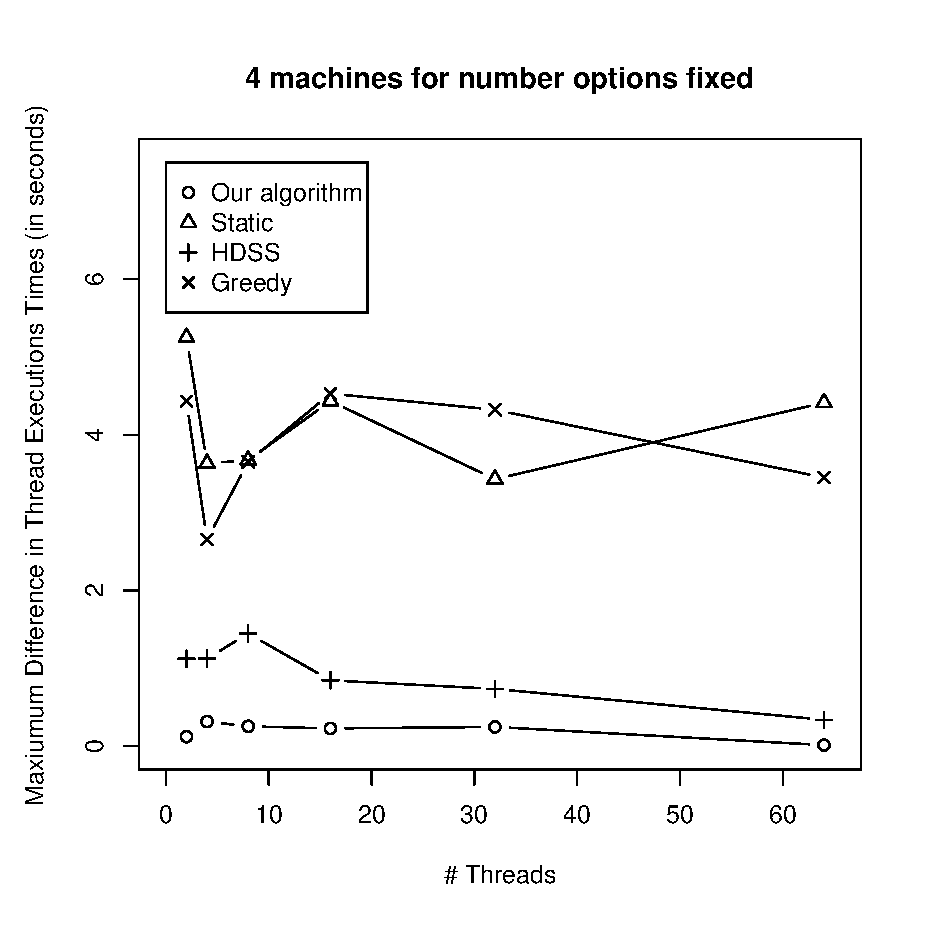
\includegraphics[scale=0.4]{Maxima_Diferenca_BlackScholes.eps}
	\caption{Time differences between the earliest and latest finishing threads}
	\label{fig:diferencaThreadsBlack}
	\end{center}
\end{figure}

Figure~\ref{fig:diferencaThreadsBlack} confirms this result, showing that the
time difference among the earliest and latest finishing threads, in the
scenario with four machines is always smaller for our proposed algorithm.


\subsection{Gene regulatory networks inference}

As in previous applications, we compare the execution time in four different environments: with  one machine, two machines, three machines and four machines. The results are shown in \ref{fig:Gene}. We can notice that our algorithm outperformed in four cases. Especially in the case that three and four machines were used. 

\begin{figure}[htb]
	\begin{center}
	\centering
			\includegraphics[scale=0.4]{GraficoFabrizio4maquinasNOVO.pdf}
	\caption{Difference in runtime with different numbers of genes for gene regulatory network inference}
	\label{fig:Gene}
	\end{center}
\end{figure}

The table \ref{table: gene} shows the extreme values​​, for 100,000 and 2,000,000 genes. 
To the environment with 3 and 4 machines the performance were similar due to limitation in data transfer, in the case of four machines the communication cost limited the gain. The total cost of calculating the distribution of the blocks is 821.54
milliseconds and standard deviation of 142.23 miliseconds.

\begin{table*}[htb]
\centering
\caption{Comparative: HDSS x Our Algorithm}

\begin{tabular}{c|c|c|c|c|c|c|}
\cline{2-7}
\multicolumn{1}{l|}{}                 & \multicolumn{3}{c|}{100,000 Genes}                              & \multicolumn{3}{c|}{2,000,000 Genes}                                                  \\ \hline
\multicolumn{1}{|l|}{Num. Machines} & HDSS (s) & Algorithm (s) & \multicolumn{1}{l|}{Diff. (\%)} & \multicolumn{1}{l|}{HDSS (s)} & Algorithm (s) & \multicolumn{1}{l|}{Diff. (\%)} \\ \hline
\multicolumn{1}{|c|}{1 }       &197.94     & 116.43              & 70.00                         & 927.43                         & 889.13              &           4.31                 \\ \hline
\multicolumn{1}{|c|}{2 }      & 79.76     & 53.43              & 49.28                            & 702.65                          & 632.73              & 11.05                           \\ \hline
\multicolumn{1}{|c|}{3 }      & 34.76     & 21.39              & 62.50                            & 502.65                          & 432.43             &               16.24                  \\ \hline
\multicolumn{1}{|c|}{4 }      & 25.91     & 18.54              & 39.75                            & 479.54                          & 411.46             &               16.54  \\ \hline
\end{tabular}
\label{table: gene}
\end{table*}

Like the other experiments, the maximum difference among the threads followed the same principle. Our algorithm has the smallest difference among the threads, figure \ref{fig:GeneDiferenca}.

\begin{figure}[htb]
	\begin{center}
	\centering
			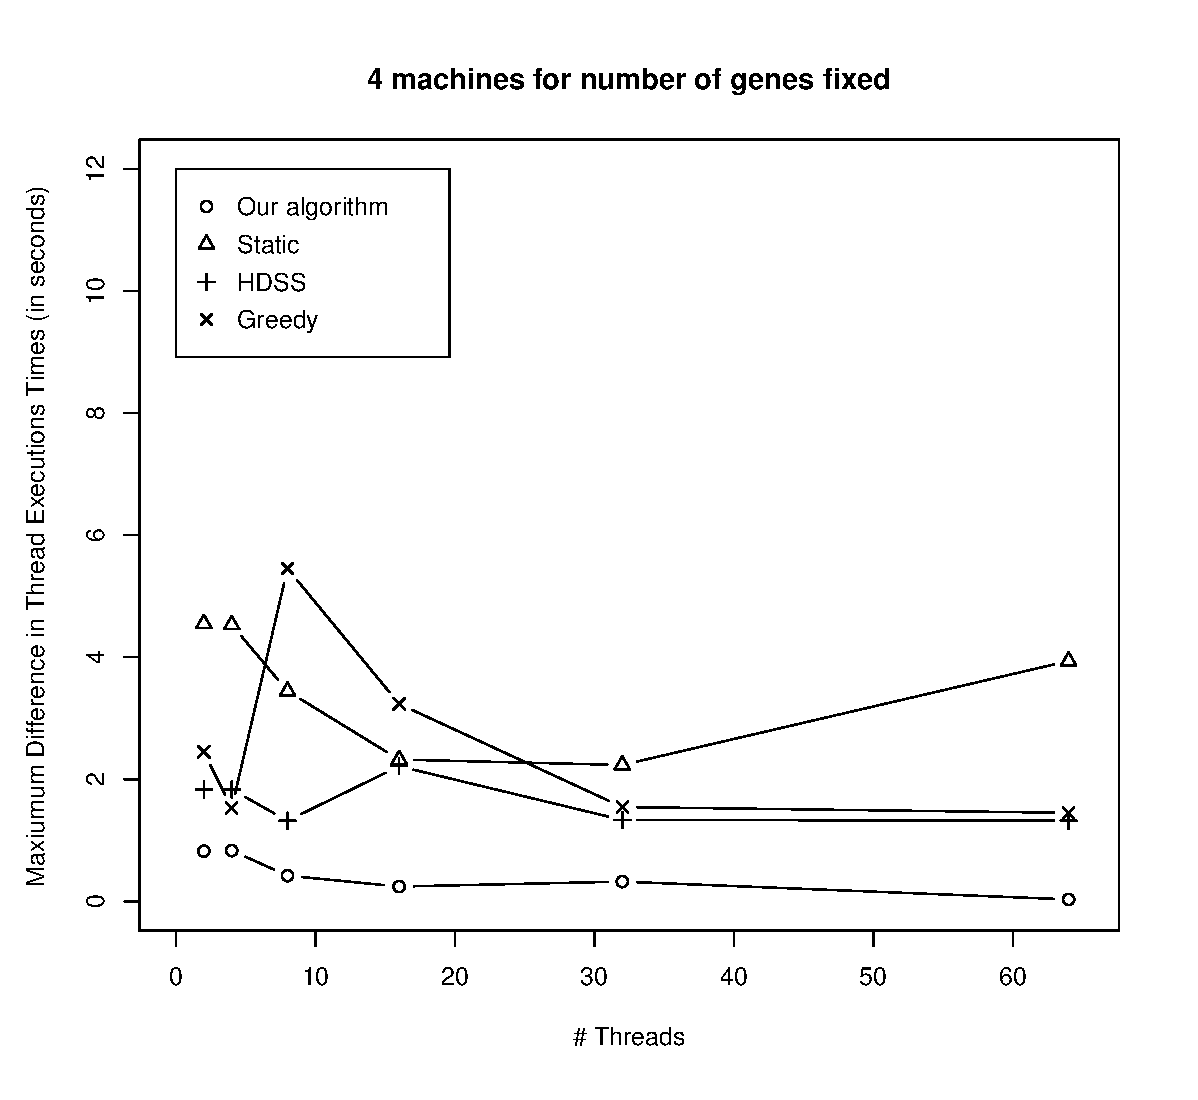
\includegraphics[scale=0.4]{Maxima_Diferenca_Fabrizio.eps}
	\caption{Difference in runtime with different numbers of genes for gene regulatory network inference}
	\label{fig:GeneDiferenca}
	\end{center}
\end{figure}

\subsection{Block size evolution}

In the figure \ref{fig:GeneBlocos} we compare the behavior in relation to
submission of blocks among machines. It analyzed the block size for the HDSS and
our algorithm. In this case three machines were used, it is possible to notice
the difference between runs. Our algorithm in step 400 suffered a re-balancing,
causing it to change the size of the block. In HDSS, a decrease of the block
size remains over the iterations.

\begin{figure}[htb]
	\begin{center}
	\centering
			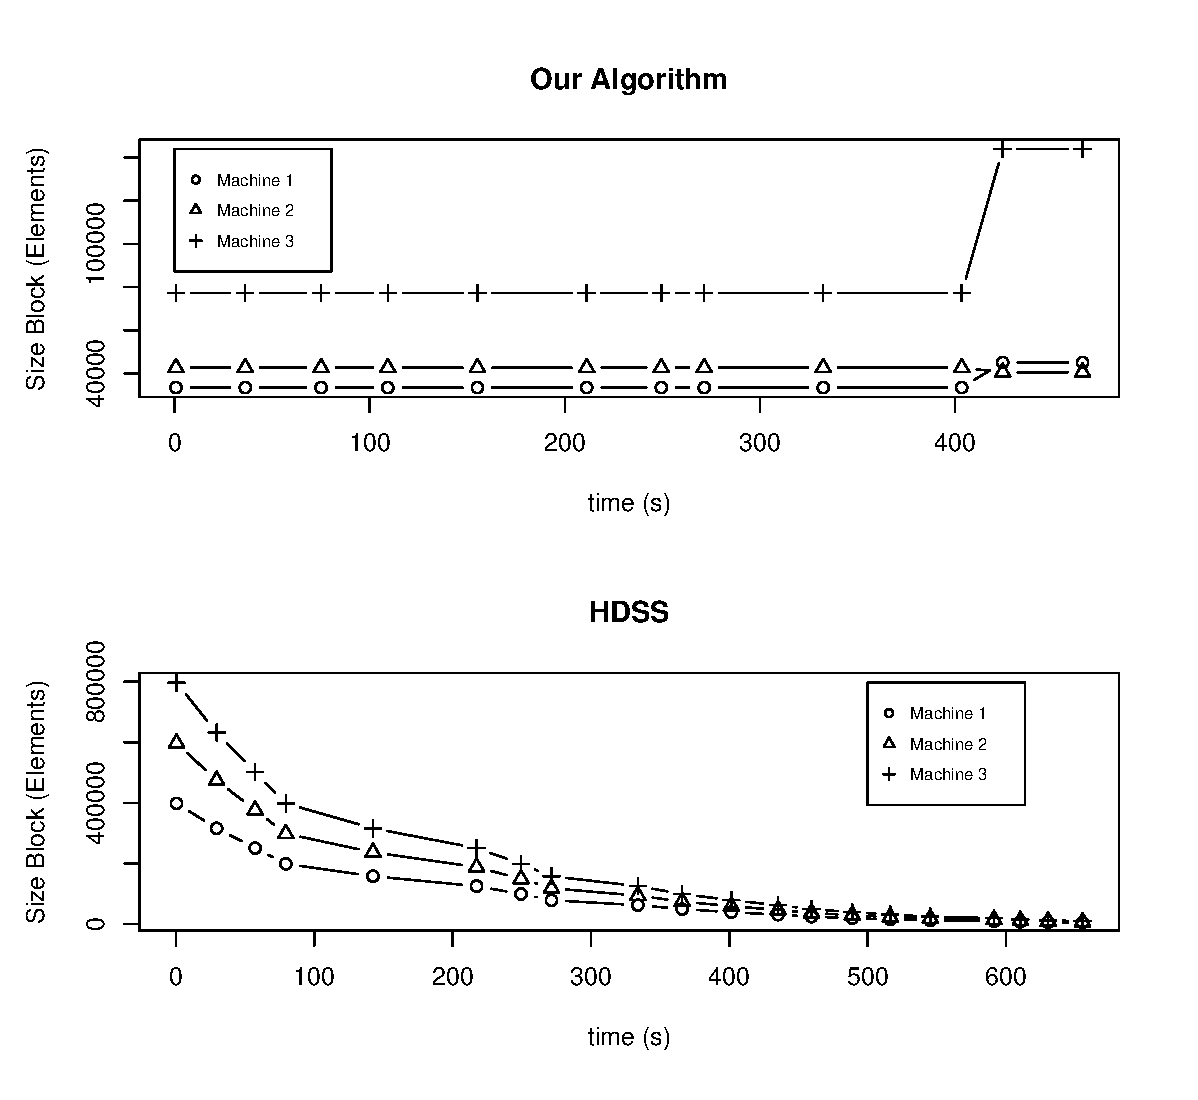
\includegraphics[scale=0.4]{BlocosComportamento_Fabrizio.eps}
	\caption{Difference in runtime with different numbers of genes for gene regulatory network inference}
	\label{fig:GeneBlocos}
	\end{center}
\end{figure}


%-------------------------------------------------------------------------------
\section{Conclusions and future work}

In this paper we propose an algorithm for scheduling tasks in domain
decomposition problems executing on clusters of heterogeneous CPUs and GPUs. It
outperforms other similar existing algorithms, due to the online estimation of
the performance curve for each processing unit and the selection of the best
data distribution for the devices. We showed for two applications that our
algorithm provides the highest gains for more heterogeneous and larger problems
sizes.

Although we used dedicated clusters, we can also consider the usage of public
clouds, where the user can request a number of resources allocated in virtual
machines from shared machines. In this case, the quality of service may change
during execution, and the addition of the execution time difference threshold
permits readjustments in data distributions. We can also consider the scenario
with added fault-tolerance, where machines may become unavailable during
execution. In this scenario, a simple redistribution of the data among the
remaining devices would permit the application to readapt to this scenario.

As ongoing work, we are including the cost of communication in the scheduling
algorithm, which is essential for applications where the time spent with
information exchange among the tasks cannot be ignored.

% use section* for acknowledgement
\section*{Acknowledgment}


The authors would like to thank FAPESP (Proc. n. 2012/03778-0 and Proc. n.  2013/14603-9) for the financial support.


\ifCLASSOPTIONcaptionsoff
  \newpage
\fi

% can use a bibliography generated by BibTeX as a .bbl file
% BibTeX documentation can be easily obtained at:
% http://www.ctan.org/tex-archive/biblio/bibtex/contrib/doc/
% The IEEEtran BibTeX style support page is at:
% http://www.michaelshell.org/tex/ieeetran/bibtex/
\bibliographystyle{IEEEtran}
% argument is your BibTeX string definitions and bibliography database(s)
%\bibliography{IEEEabrv,../bib/paper}
%
% <OR> manually copy in the resultant .bbl file
% set second argument of \begin to the number of references
% (used to reserve space for the reference number labels box)
% File .bib
\bibliography{article}


\end{document}


